
\subsection{Results}

Unless otherwise specified,
I analysed the data using linear or logistic mixed models,
with random intercepts for each participant,
and random coefficients for the effect of condition for each participant.

Participants reasoning about generic properties
gave the foil response on
none of the control trials (N = 190),
but on 46\% of the conflict trials.
Those reasoning about specific properties
gave the foil response on 4\% of control trials,
and on 17\% of conflict trials
(see Table~\ref{tab:exp2_responses}).
A 2 (condition) x 2 (properties) logistic mixed model%
\footnote{
  Once again, as all participants gave the correct response
  in the control condition with generic properties,
  I used penalised maximum likelihood to set a normal prior,
  with mean 0 and SD 3, on the regression coefficients here \citep{Zorn2005}.
  This model also omitted the random coefficients
  for the effect of condition for each participant,
  due to convergence issues.
}
found a main effect of condition
($e^{\beta}$ = 95.7, CI = [28.6; 320.0],
z = 7.403, p < .0001),
and a condition x properties interaction
($e^{\beta}$ = 74.2, CI = [7.5; 730.4], z = 3.691, p < .0001),
such that the effect of condition was more pronounced
for participants reasoning about generic properties.

\begin{table}
  \centering
  \begin{tabular}{lrrr}
    \toprule
    \multicolumn{1}{l}{}          &
    \multicolumn{2}{l}{Condition} &
    \multicolumn{1}{l}{} \\
    \cmidrule(lr){2-4}
    Properties & Control & Conflict & Mean \\
    \midrule

    Specific   &    4\%  &    17\%  &  10\%  \\
    Generic    &    0\%  &    46\%  &  23\%   \\
    \midrule
    Mean       &    2\%  &    32\%  &        \\
    \bottomrule
  \end{tabular}
  \caption{
    Foil responses in Experiment 2.
    \label{tab:exp2_responses}
  }
\end{table}

Figure~\ref{fig:exp2_acc} shows how this effect was distributed across participants.
Recall that participants completed eight reasoning trials in each condition.
Of the 22 participants reasoning about generic properties,
16 were more likely to give the foil response under conflict,
none were more likely to do so on control trials,
and 8 never gave the foil response.
Of the 22 reasoning about specific properties,
11 were more likely to give the foil response under conflict,
2 more likely to do so on control trials,
and 11 never chose the foil option.
Therefore, as in Experiment 1, the main effect does not appear
to be driven by an effect only a subset of participants.

\begin{figure}[ht]
  \centering
  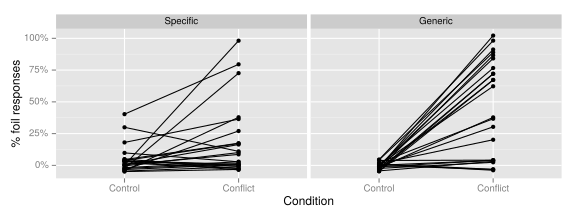
\includegraphics[width=\figurewidth]{imgs/exp2_acc.pdf}
  \caption[Proportion of foil responses given by each participant, per condition, in Experiment 2.]{
    Proportion of foil responses given by each participant per condition, in Experiment 2.
    separately for each property type.
    A small jitter has been added to vertical positions
    to show points which would otherwise overlap.
    \label{fig:exp2_acc} }
\end{figure}


\begin{table}
  \centering
  \begin{tabular}{llrrrr}
    %% Despace me!
   \toprule
    Properties                & Condition & Foil choices &  RT (msec)    & IT (msec) &  Reversals\\
    \midrule
    \multirow{2}{*}{Specific} & Control   &   4\%        &  1,366 (964)  & 377 (254) &  16\%\\
                              & Conflict  &   17\%       & 1,611 (1,162) & 362 (181) &  52\%\\
    \multirow{2}{*}{Generic}  & Control   &  0\%         &  1,547 (912)  & 444 (389) &  11\%\\
                              & Conflict  &   46\%       &  2,121 (1293) & 509 (576) &  59\%\\
    \bottomrule
  \end{tabular}
  \caption[Descriptive statistics for correct responses, Experiment 2.]{
    Summary statistics for correct responses, by property type and condition,
    on the odds of participants selecting the foil option (foil choices),
    and summary statistics for correct responses: response time (RT),
    movement initiation time (IT),
    and number of reversal trajectories (Reversals).
    \label{tab:exp2_descriptive}
  }
\end{table}


%% \begin{table}
%%   \centering
%%   \begin{tabular}{llllll}
%%     \toprule
%%                            & Foil choices & RT        & IT    &  Reversals\\
%%     \midrule
%%     Condition              & 95.7 ***     & 130\% *** & 102\% & 9.3 ***\\
%%     Properties             & 1.0          & 125\% **  & 114\% & 0.9\\
%%     Condition x Properties & 74.2 ***     & 119\% *   & 119\% & 1.7\\
%%     \bottomrule
%%     \multicolumn{5}{l}{ \emph{Note}: $^{*} p < .05;\ ^{**} p < .01;\ ^{***} p < .001;\ ^{****} p < .0001$ }
%%   \end{tabular}
%%   \caption{
%%     $e^{\beta}$ regression weights (odds ratio change for binary outcomes,
%%     and percentage change in log-transformed continuous outcomes,
%%     for main effects of condition and property type,
%%     and their interaction for each measure.
%%     Weights greater than 1/100\% indicate
%%     an increase in the dependent variable on conflict trials for the effect of condition,
%%     and increase for generic properties for the effect of properties,
%%     and an increase in the effect of condition when reasoning about generic properties
%%     for the interaction term.
%%   }
%% \end{table}

As in Experiment 1, IT did not differ significantly
between conditions or property types (p's > .2).
Response times were in general slower in the conflict condition (1,815 msec, SD = 1,239)
than the control condition (1,458 msec, SD = 941;
$e^{\beta}$ = 130\%, CI = [120\%; 140\%],
t(186.54) = 7.057, p < .0001),
and slower for generic properties (1,747 msec, SD = 1,094)
than specific properties (1478 msec, SD = 1,064;
$e^{\beta}$ = 125\%, CI = [106\%, 146\%],
t(46.1) = 2.731, p = .0089).
There was a significant condition x property interaction,
such that the effect of condition
was more pronounced for generic properties
($e^{\beta}$ = 119\%, CI = [103\%; 138\%],
t(186.4) = 2.382, p = .0182).

MD was bimodally distributed
(Bimodality coefficient = .635,
Hartigan's D = 0.02, p = .0341),
and so trajectories with MD greater than 0.747 were categorised as reversals
(see Appendix~\ref{appendix:reversals}).
For correct responses, these reversals occurred
significantly more often for conflict trials (61\% of trials)
than for control trials (17\% of trials;
$e^{\beta}$ = 9.2, CI = [6.0; 14.2], z = 10.21, p < .0001),
with no effect of property type, or condition x property interaction.

\begin{table}
  \centering
  \begin{tabular}{ll R{1.8cm} R{1.8cm} R{1.8cm} R{1.8cm} }
    \toprule
    Properties                & Condition & Direct Correct & Reversal Correct & Reversal Foil & Direct Foil\\
    \midrule
    \multirow{2}{*}{Specific} & Control   & 77.4\%         & 18.9\%           & 2.1\%         & 1.6\%\\
                              & Conflict  & 33.0\%         & 49.7\%           & 4.9\%         & 12.4\%\\
    \multirow{2}{*}{Generic}  & Control   & 85.8\%         & 14.2\%           & 0\%           & 0\%\\
                              & Conflict  & 20.6\%         & 33.3\%           & 12.2\%        & 33.9\%\\
    \bottomrule
  \end{tabular}
  \caption[Kinds of trajectory in Experiment 2.]{
    The prevalence of each kind of mouse trajectory, by condition and property type.
    \label{tbl:exp2_trajectories}}
\end{table}

There were therefore, once again, four kinds of cursor trajectories:
Direct Correct, Reversal Correct, Reversal Foil, and Direct Foil trajectories.
Table~\ref{tbl:exp2_trajectories} shows the proportion of each trajectory type,
broken down by condition and property type.
Across both property types,
participants were less likely to go straight to the correct option and choose it,
and more likely to do so for the foil option, under conflict.
In line with the analysis of reversals above,
initial movements towards the foil, which redirect to choose the correct option,
were more common under conflict,
and this difference was more pronounced for specific properties,
while this manipulation made participants reasoning about generic properties
more likely to instead give the foil response.



\begin{table}
  \centering
  \begin{tabular}{llccc}
    \toprule
    %%                        &            & \multicolumn{3}{c}{Parameter}\\
    Condition                    & Properties & $\alpha$             & $\beta$ & $\gamma$\\
    \midrule
    \multirow{3}{*}{Control}     & Specific   & 80\%                 & 97\%    & 92\%\\
                                 & Generic    & 86\%                 & 100\%   & 100\%\\
    \cmidrule(lr){2-5}
                                 & Both       & 83\%                 & 99\%    & 96\%\\
                              %% & Both       & \circled[blue]{83\%} & 99\%    & 96\%\\
    \midrule
    \multirow{3}{*}{Conflict}    & Specific   & 38\%                 & 87\%    & 80\%\\
                                 & Generic    & 33\%                 & 63\%    & 50\%\\
    %% \multirow{3}{*}{Conflict} & Specific   & 38\%                 & 87\%    & \circled{80\%}\\
    %%                           & Generic    & 33\%                 & 63\%    & \circled{50\%}\\
    \cmidrule(lr){2-5}
                                 & Both       & 35\%                 & 76\%    & 64\%\\
                              %% & Both       & \circled[blue]{35\%} & 76\%    & 64\%\\
    \bottomrule
  \end{tabular}
  \caption[Transition probabilities for Experiment 2.]{
    Transition probabilities for Experiment 2.
    Regardless of property type, participants are more likely
    to initially move towards the correct option ($\alpha$),
    and to ultimately select the correct option,
    either after initially moving towards it ($\beta$)
    or after initially moving towards the foil ($\gamma$)
    on control trials, where the correct option and the base look alike.
    On conflict trials, participants who initially moved towards the foil option
    were more likely to ultimately select the correct option instead ($\gamma$)
    when reasoning about specific properties than
    when reasoning about generic properties.
    Participants were initially less likely to move
    towards the correct option on conflict trials (blue),
    and after initially moving towards the foil on conflict trials,
    they were more likely to change direction and select the correct option
    if reasoning about specific properties than generic (red).
  }\label{tbl:exp2_transitions_table}
\end{table}


We can better understand these effects, once again,
by turning to the transition probabilities.
Table~\ref{tbl:exp2_transitions_table} shows
these transition probabilities,
broken down by condition and by property type.
I analysed these probabilities
using 2 (condition) x 2 (properties) logistic mixed models,
with random intercept terms for each participant.
Initial movements to the correct response,
with probability $\alpha$, were significantly more common for control trials (82.6\%)
than conflict trials (32.3\%;
$e^{\beta}$ = 10.1, CI = [7.0; 14.6], z = 2.312, p < .0001),
but with no main effect of property type.
A marginally significant condition x property interaction
($e^{\beta}$ = 2.0, CI = [0.9; 4.0], z = 1.904, p = .0569)
indicated that the effect of condition on $\alpha$
was slightly more pronounced for generic properties.

For trials where participants initially moved towards the correct option,%
\footnote{
  Again, in both the analysis of $\beta$ and $\gamma$,
  as means of 0 and 1 occurred in a number of cells,
  penalised maximum likelihood logistic regression was used,
  with a Gaussian prior (mean 0, SD 3) on each regression coefficient.
  }
the probability of ultimately selecting the correct option ($\beta$)
was greater in control trials (98.7\%) than conflict trials (75.8\%;
$e^{\beta}$ = 46.1, CI = [11.6; 182.9], z = 5.453, p < .0001).
There was no main effect of property type,
but there was a significant property x condition interaction
($e^{\beta}$ = 47.1, CI = [3.7; 601.5], z = 3.692, p = .0030),
such that the effect of condition for generic properties
was greater than that for specific properties.
It should be noted, however, that $\beta$ was largely positive.
Even on conflict trials, with generic properties,
participants who initially moved towards the correct option
ended up selecting in 63\% of the time.

For the trajectories that initially moved towards the foil,
the probability of changing direction and ultimately selecting the correct option ($\gamma$),
was lower for conflict trials (64\%)
than control trials (95\%;
$e^{\beta}$ = 34.4, CI = [7.1; 166.2], z = 4.402, p < .0001).
There was no main effect of property types, but
there was, crucially, a property x condition interaction
($e^{\beta}$ = 66.6, CI = [3.8; 1149.1], z = 2.890, p = .0039),
indicating that the effect of condition was greater
for participants reasoning about generic properties.
Post-hoc comparisons showed no difference
between participants reasoning about specific and generic properties
in the control condition ($\gamma$ > 92\%; $p_{adjusted}$ > .4),
but significantly more correct responses
after initially moving towards the foil option on conflict trials
when reasoning about specific properties (80\%)
than when reasoning about generic properties (50\%;
$e^{\beta} = 19.2, CI = [2.1, 174.5], z = 2.622, p_{adjusted} = .0088$.






In Experiment 1, I found that initial movements towards the foil option on conflict trials
were initiated more quickly than those towards the correct option.
Here, I fitted a 2 (initial movement direction) x 2 (property type) logistic mixed model,
with random intercepts for each participant and each base species,
and log-transformed initiation times from the conflict trials as the dependent variable.
There was a significant effect of initial direction,
such that movements towards the foil option (430 msec, SD = 527)
were again initiated faster than movements towards the correct option (558 msec, SD = 564;
$e^{\beta}$ = 118\%, CI = [1.07\%, 131\%], t(346.2) = 3.325, p = .0010).
There was no effect of property type, or condition by property interaction ($p's > .1$).


\subsubsection{Time course}

I repeated the time course analysis reported for Experiment 1,
looking at the proportion of trials on the side of the screen
corresponding to each response option over time.
Firstly, Figure~\ref{fig:exp2_foil_side_timecourse}
shows the proportion of trials on the side of the screen
containing the foil option, over time,
broken down by condition, and property type.
To infer when each variable began to influence participants' motor output,
I fitted a series of logistic mixed models,
predicting the proportion of responses on the foil side of the screen
at each 20 msec interval.
To test the effect of condition, I fitted models
with condition as a predictor, and random intercepts for each participant.
To investigate the effect of properties,
I fitted models with property as a predictor, and random intercepts for each participant,
to the data from conflict trials only,
as control trials were unaffected by manipulations of the property.
Participants were more likely to
move toward the foil option in conflict trials than control trials from 280 msec
(solid vertical line in Figure~\ref{fig:exp2_foil_side_timecourse}).
On conflict trials, participants reasoning about generic properties
were more likely to remain on the foil side of the screen than those 
reasoning about specific properties from 620 msec (dashed vertical lines).
In other words, participants reasoning about specific properties
were more likely to override their movement towards the foil from this point.


\begin{figure}[tp]
  \centering
  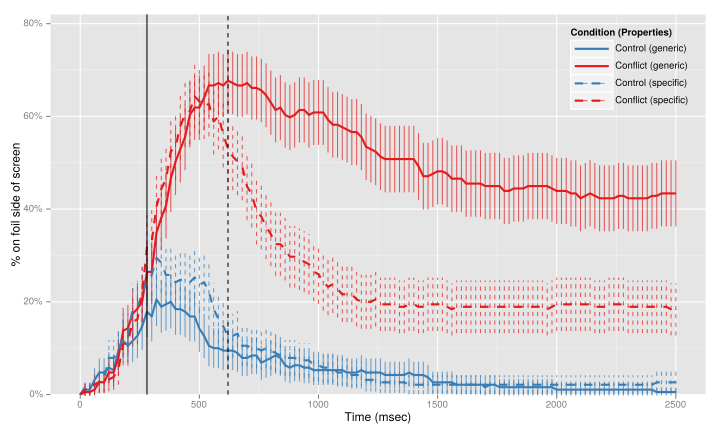
\includegraphics[width=\figurewidth]{imgs/exp2_foil_side_timecourse.pdf}
  \caption[Time course of attraction towards the foil, in Experiment 2.]{
    \label{fig:exp2_foil_side_timecourse}
    Proportion of trials on the side of the screen containing the foil option, over time.
    Participants were more drawn towards the foil option
    early in conflict trials (red) than control trials (blue)
    from  260 msec (solid vertical line).
    Later on conflict trials, participants were  more likely to remain on the foil side
    when reasoning about generic properties (solid red line)
    than specific properties (dashed red line),
    from 620 msec (dashed vertical line).
  }
\end{figure}

\begin{figure}[bp]
  \centering
  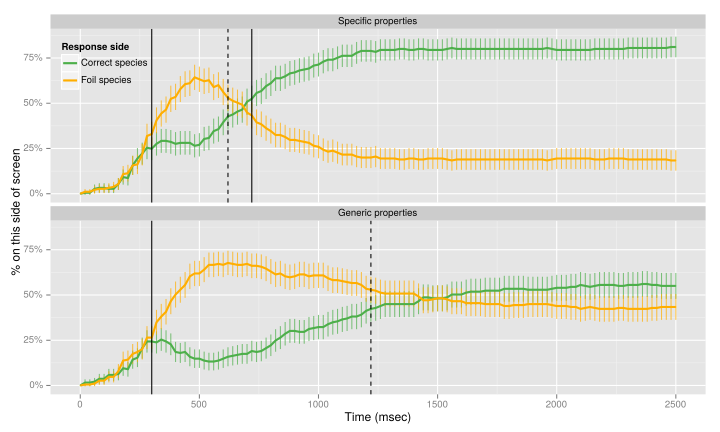
\includegraphics[width=\figurewidth]{imgs/exp2_conflict_timecourse.pdf}
  \caption[Time course for conflict trials, in Experiment 2.]{
    Time course of attraction towards foil and correct response options
    on conflict trials with generic (top) and specific (bottom) properties.
    Participants reasoning about both kinds of property
    show an early preference for the foil option
    (statistically significant from the first solid vertical lines to the dashed vertical lines)
    which is inhibited quickly for specific properties,
    and more slowly, and less often, for generic properties.
    Only participants reasoning about specific properties
    showed a later significant preference for the correct option (second solid vertical line).
    \label{fig:exp2_conflict_timecourse} }
\end{figure}

Figure~\ref{fig:exp2_conflict_timecourse} shows, for conflict trials,
the proportion of trials on the side of the screen corresponding to each response.
The top panel shows these trends for participants reasoning about specific properties.
Participants were significantly more likely to be on the side of the foil option than the correct option
from 300 msec (first solid vertical line) to 620 (vertical dashed line),
and subsequently significantly more likely to be on the side of the correct option
from 720 msec onwards (second solid vertical line).
The bottom panel, for participants reasoning about generic properties, shows a similar trend.
Participants were again significantly more likely to be on the side of the foil option
from 300 msec (first solid vertical line),
but this initial effect persevered for much longer when reasoning about generic properties,
to 1,220 msec (vertical dashed line),
and participants never showed a significant preference
for the correct option's side of the screen.

Therefore, participants reasoning about both kinds of property
were initially driven by perceptual cues in the conflict condition,
but those reasoning about specific properties
were more likely than those reasoning about generic properties
to subsequently draw on conceptual knowledge
and move instead to the side of the screen
containing the correct response option,
and were faster to do so.

\FloatBarrier
